%pdf-latex

%header nur vom MÜSLI-Vortrag geklaut
% !TEX root = vortrag.tex
% !TEX encoding = UTF-8 Unicode

\documentclass[t, ngerman]{beamer} %compress,

%% Pakete laden...
  \usepackage[T1]{fontenc}
  \usepackage[utf8]{inputenc}
  \usepackage{
      babel,
      bookmark,
      booktabs,
%      blindtext,
      colortbl,
%      eurosym,
      graphicx,
	  hyperref,
%      libertine,
      microtype,
      pifont,
      pgfpages,
      tikz,
%      xspace,
  }


%% Design festlegen...
  \mode<presentation>{
%      \useoutertheme[subsection=false]{smoothbars}
      \useinnertheme{rectangles} % rectangles, circles, rounded
      \usecolortheme[RGB={153,0,0}]{structure}
      \definecolor{unihd}{RGB}{153,0,0}
      \definecolor{dark}{RGB}{115,0,0}
      \definecolor{light}{RGB}{241,229,229}
      \usecolortheme{whale}
		 \usecolortheme{orchid}
%	   \usecolortheme{beaver}
%      \setbeamercovered{transparent}
      \beamertemplatenavigationsymbolsempty
%      \setbeameroption{show notes on second screen}
      \setbeamertemplate{note page}[plain]
      \logo{
\includegraphics[width=3.5cm]{fs-logo-small}}

  }

%% nützliche Definitionen...
  \graphicspath{{media/}}

%% Titelinformationen...
  \title[Studienverwaltung$\mu$]{Das Müsli und das LSF\\\small oder: wer wie was wo Stundenplan}
  \author[
	koebi
  ]{
	Jakob Schnell\\{\scriptsize\url{koebi@mathphys.stura.uni-heidelberg.de}}
  }
%  \institute{  
\includegraphics[width=5.5cm]{fs-logo-big} }

  \date{\vspace*{-2em}\\ 01. Oktober 2018}

  \hypersetup{
      pdfauthor={Jakob Schnell},
      pdftitle={Müsli-Vortrag},
      pdfsubject={hihi},
      pdfkeywords={1},
      pdfpagelayout={SinglePage},
  }
  


\newenvironment{rcases}{%
  \left.\renewcommand*\lbrace.%
  \begin{cases}}%
{\end{cases}\right\rbrace}


\begin{document}

\begin{frame}[fragile]
    \maketitle
\end{frame}

\begin{frame}[fragile]{Inhalt}
    \tableofcontents[hideallsubsections]
\end{frame}

%%%%%%%%%%%%%%%%%%%%%%%%%%%%%%%%%%%%%%%%%%%%%%%%%%%%%%%%%%%%
% Digitale Infrastruktur
%%%%%%%%%%%%%%%%%%%%%%%%%%%%%%%%%%%%%%%%%%%%%%%%%%%%%%%%%%%%

\section{Digitale Infrastruktur}
\begin{frame}{Digitale Infrastruktur}
    \large
    \begin{itemize}
        \item{WLAN}
        \item{VPN}
        \item{Drucken}
        \item{CIP-Pool}
        \item{Uni-Mail-Adresse}
    \end{itemize}
\end{frame}

%%%%%%%%%%%%%%%%%%%%%%%%%%%%%%%%%%%%%%%%%%%%%%%%%%%%%%%%%%%%
% WLAN
%%%%%%%%%%%%%%%%%%%%%%%%%%%%%%%%%%%%%%%%%%%%%%%%%%%%%%%%%%%%

\subsection{WLAN}
\begin{frame}{WLAN}
\end{frame}

%%%%%%%%%%%%%%%%%%%%%%%%%%%%%%%%%%%%%%%%%%%%%%%%%%%%%%%%%%%%
% VPN
%%%%%%%%%%%%%%%%%%%%%%%%%%%%%%%%%%%%%%%%%%%%%%%%%%%%%%%%%%%%

\subsection{VPN}
\begin{frame}{VPN}
\end{frame}

%%%%%%%%%%%%%%%%%%%%%%%%%%%%%%%%%%%%%%%%%%%%%%%%%%%%%%%%%%%%
% Drucken
%%%%%%%%%%%%%%%%%%%%%%%%%%%%%%%%%%%%%%%%%%%%%%%%%%%%%%%%%%%%

\subsection{Drucken}
\begin{frame}{Drucken}
\end{frame}

%%%%%%%%%%%%%%%%%%%%%%%%%%%%%%%%%%%%%%%%%%%%%%%%%%%%%%%%%%%%
% CIP-Pool
%%%%%%%%%%%%%%%%%%%%%%%%%%%%%%%%%%%%%%%%%%%%%%%%%%%%%%%%%%%%

\subsection{CIP-Pool}
\begin{frame}{CIP-Pool}
\end{frame}

%%%%%%%%%%%%%%%%%%%%%%%%%%%%%%%%%%%%%%%%%%%%%%%%%%%%%%%%%%%%
% Uni-Mail-Adresse
%%%%%%%%%%%%%%%%%%%%%%%%%%%%%%%%%%%%%%%%%%%%%%%%%%%%%%%%%%%%

\subsection{Uni-Mail-Adresse}
\begin{frame}{Uni-Mail-Adresse}
\end{frame}

%%%%%%%%%%%%%%%%%%%%%%%%%%%%%%%%%%%%%%%%%%%%%%%%%%%%%%%%%%%%
% Wichtige Websites
%%%%%%%%%%%%%%%%%%%%%%%%%%%%%%%%%%%%%%%%%%%%%%%%%%%%%%%%%%%%

\section{Wichtige Websites}
\begin{frame}{Wichtige Websites}
    Die wichtigsten Websites im Unikontext sind:
    \begin{itemize}
        \item{LSF}
        \item{MÜSLI}
        \item{Moodle}
        \item{MaMpf}
    \end{itemize}
\end{frame}

%%%%%%%%%%%%%%%%%%%%%%%%%%%%%%%%%%%%%%%%%%%%%%%%%%%%%%%%%%%%
% LSF
%%%%%%%%%%%%%%%%%%%%%%%%%%%%%%%%%%%%%%%%%%%%%%%%%%%%%%%%%%%%

\subsection{LSF}
\begin{frame}{Das LSF -- Lehre, Studium und Forschung}

    \url{https://lsf.uni-heidelberg.de}

    \begin{center}
    \qrcode{https://lsf.uni-heidelberg.de}
    \end{center}

    \begin{itemize}
        \item{Veranstaltungssuche}
        \item{Studienbescheinigung}
        \item{Rückmeldung}
        \item{Bafög-Daten}
        \item{Noten}
        \item{Stundenplan}
    \end{itemize}
\end{frame}

\begin{frame}{Veranstaltungssuche}
    \begin{figure}
        \centering
        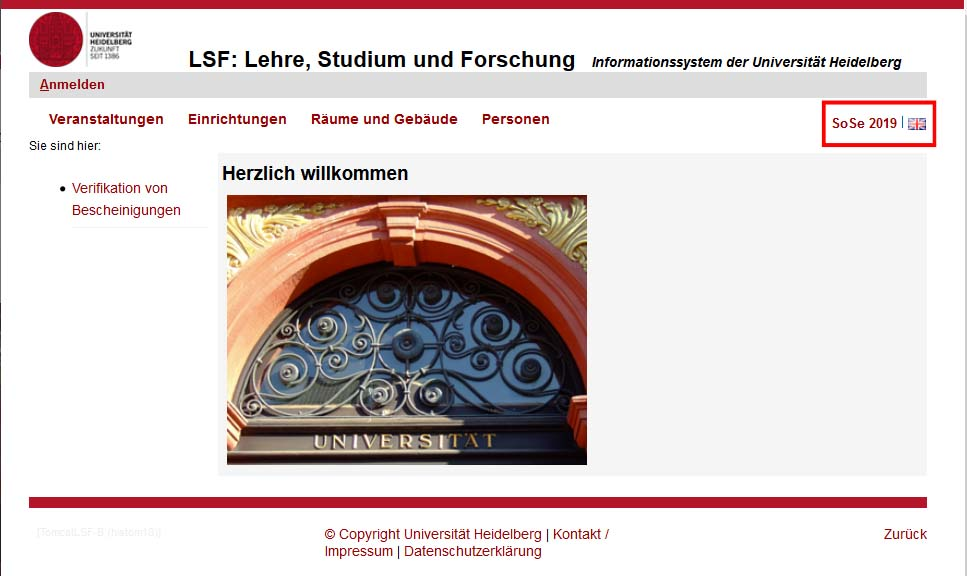
\includegraphics[scale=0.3]{images/lsf01.jpg}
    \end{figure}
Achtet darauf, dass das richtige Semester eingestellt ist, bevor ihr nach Veranstaltungen sucht.
\end{frame}

\begin{frame}{Veranstaltungssuche}
    \begin{figure}
        \centering
        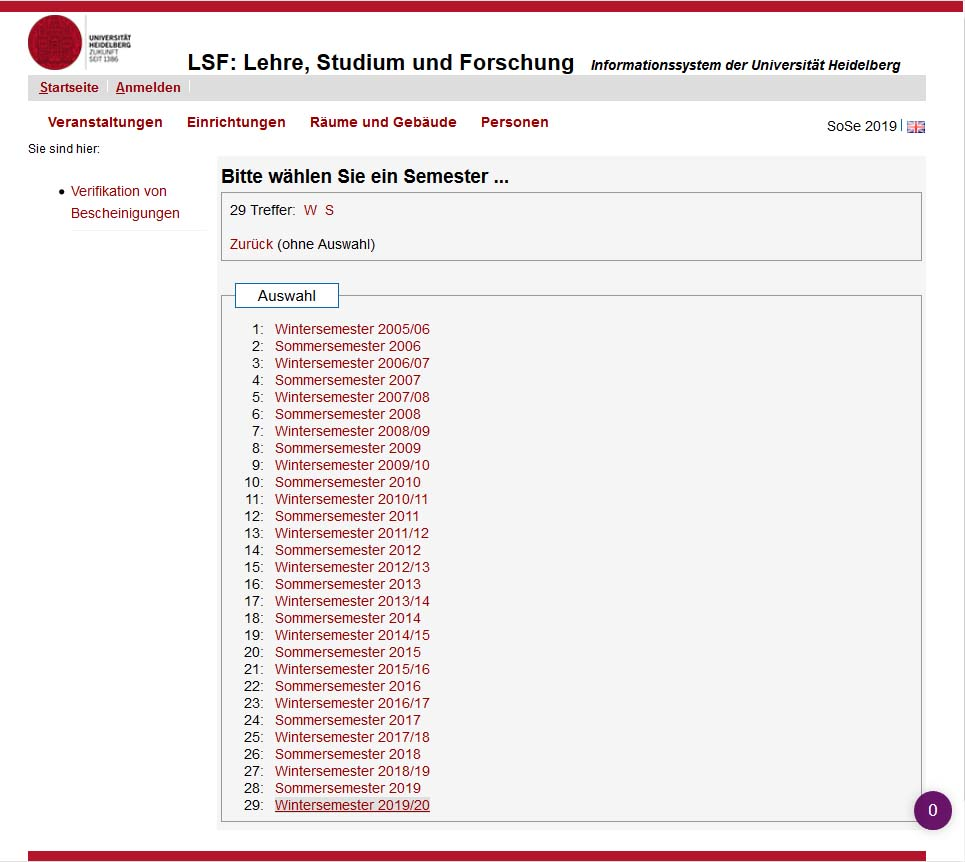
\includegraphics[scale=0.25]{images/lsf02.jpg}
    \end{figure}
\end{frame}

\begin{frame}{Veranstaltungssuche}
    Zwei Möglichkeiten, nach Veranstaltungen zu suchen
    \begin{enumerate}
        \item{Veranstaltungsangebot einer Fakultät durchsuchen (Was wird angeboten?)}
        \item{Nach konkreter Veranstaltung über die Suchfunktion suchen (Wird eine bestimmte Veranstaltung angeboten? Wann und wo findet sie statt?)}
    \end{enumerate}
    \vspace{1cm}
    Welche Veranstaltungen ihr belegen müsst/könnt, entnehmt ihr dem Modulhandbuch zu eurem Studiengang. Dazu wird es einen gesonderten Vortrag geben.
\end{frame}

\begin{frame}{Veranstaltungssuche über Fakultät, Fach, Studiengang}
    \begin{figure}
        \centering
        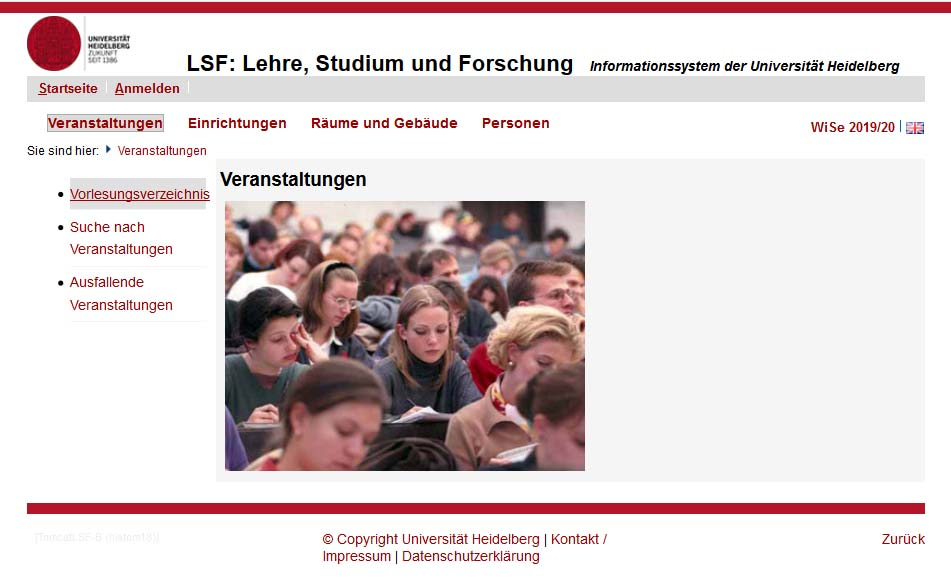
\includegraphics[scale=0.3]{images/lsf03.jpg}
    \end{figure}
\end{frame}

\begin{frame}{Veranstaltungssuche über Fakultät, Fach, Studiengang}
    \begin{figure}
        \centering
        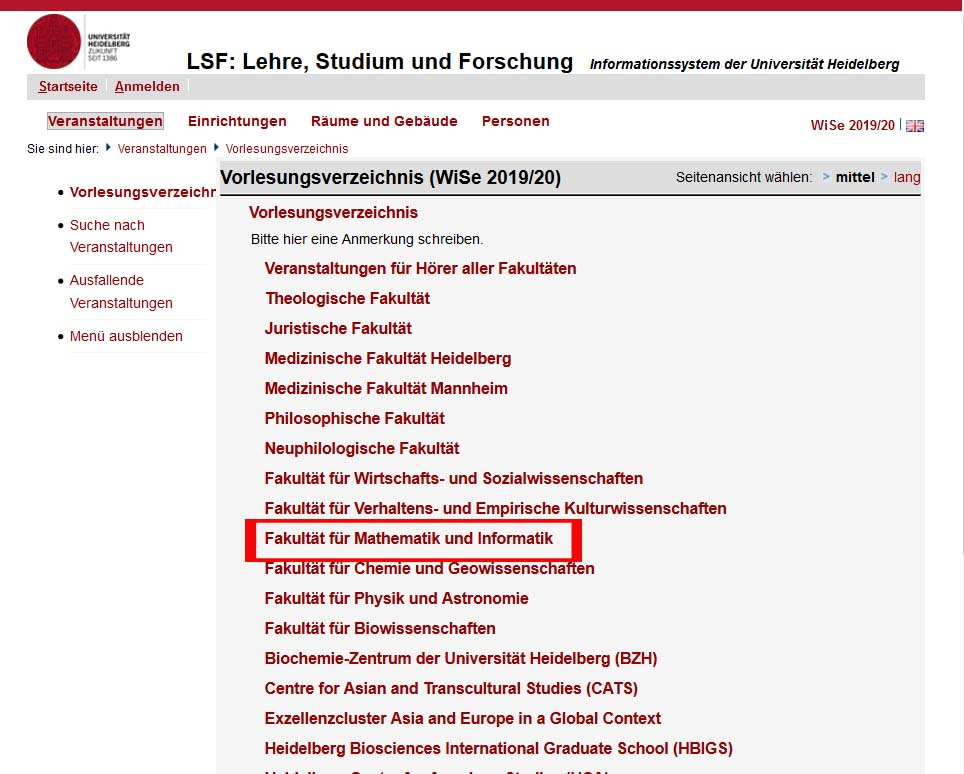
\includegraphics[scale=0.25]{images/lsf04.jpg}
    \end{figure}
\end{frame}

\begin{frame}{Veranstaltungssuche über Fakultät, Fach, Studiengang}
    \begin{figure}
        \centering
        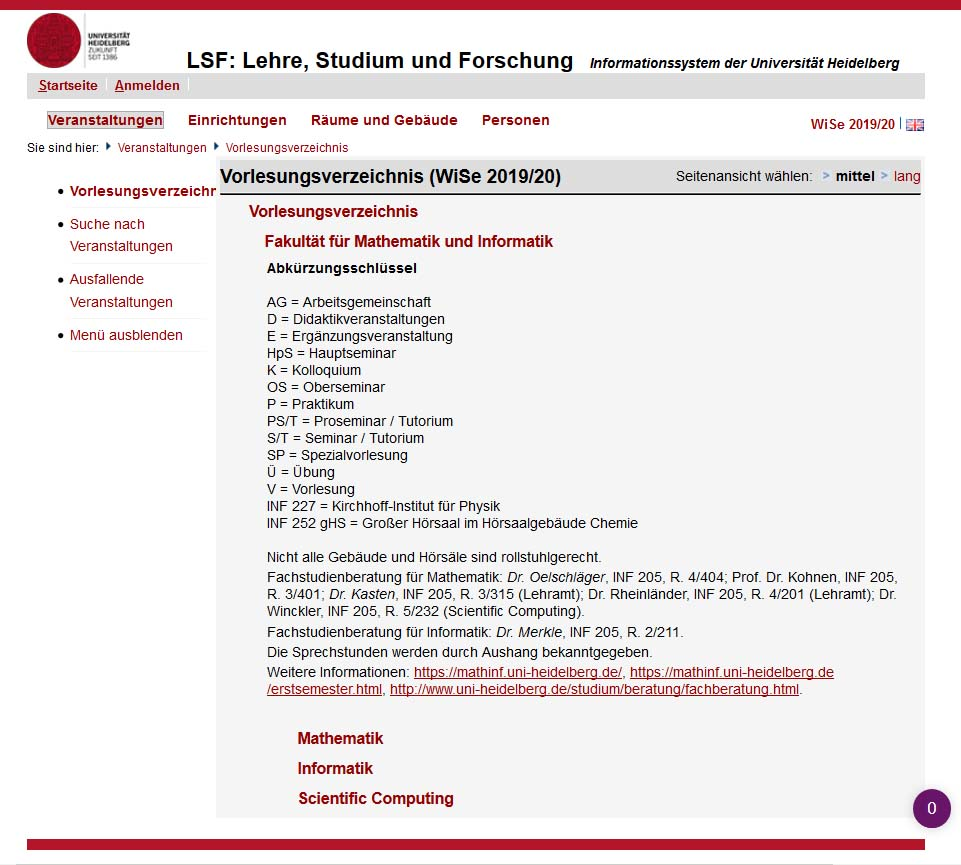
\includegraphics[scale=0.25]{images/lsf05.jpg}
    \end{figure}
\end{frame}

\begin{frame}{Veranstaltungssuche über Fakultät, Fach, Studiengang}
    \begin{figure}
        \centering
        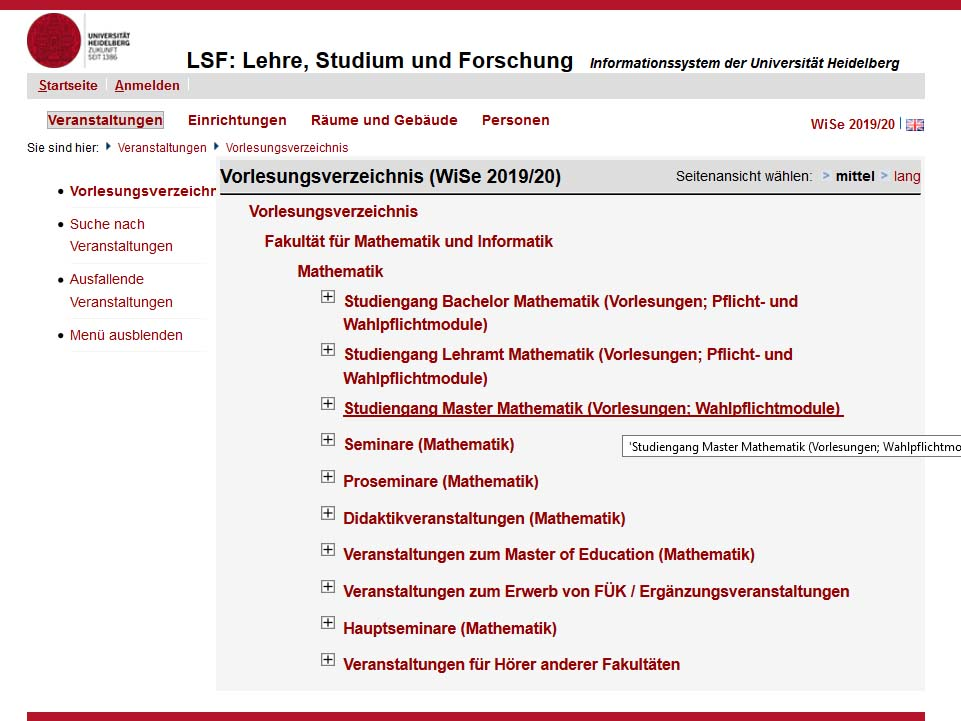
\includegraphics[scale=0.25]{images/lsf06.jpg}
    \end{figure}
\end{frame}

\begin{frame}{Veranstaltungssuche über Fakultät, Fach, Studiengang}
    \begin{figure}
        \centering
        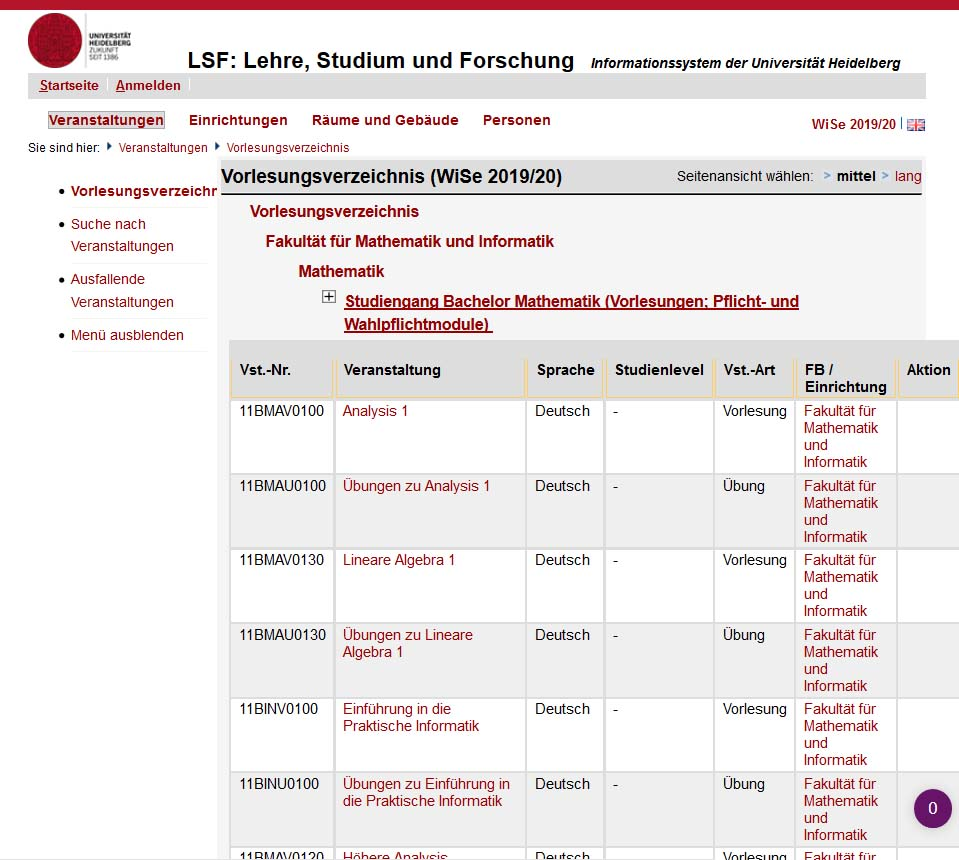
\includegraphics[scale=0.25]{images/lsf07.jpg}
    \end{figure}
\end{frame}

\begin{frame}{Veranstaltungssuche über Fakultät, Fach, Studiengang}
    \begin{figure}
        \centering
        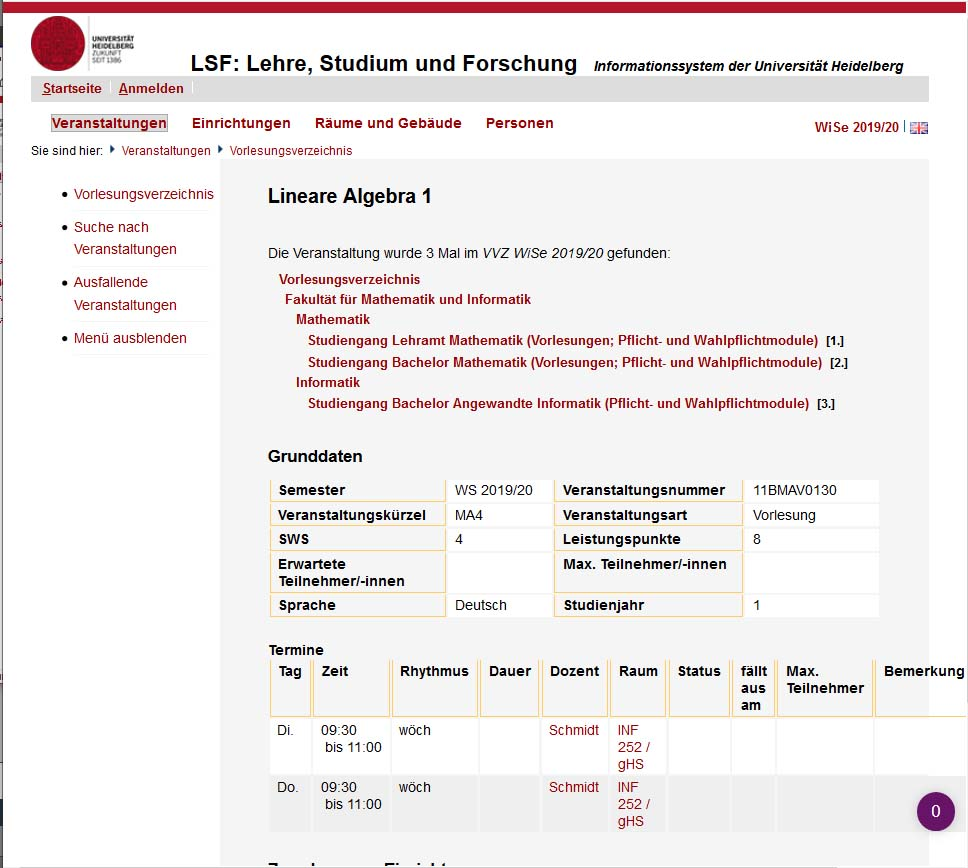
\includegraphics[scale=0.25]{images/lsf08.jpg}
    \end{figure}
\end{frame}

\begin{frame}{Veranstaltungssuche über die Suchfunktion}
    \begin{figure}
        \centering
        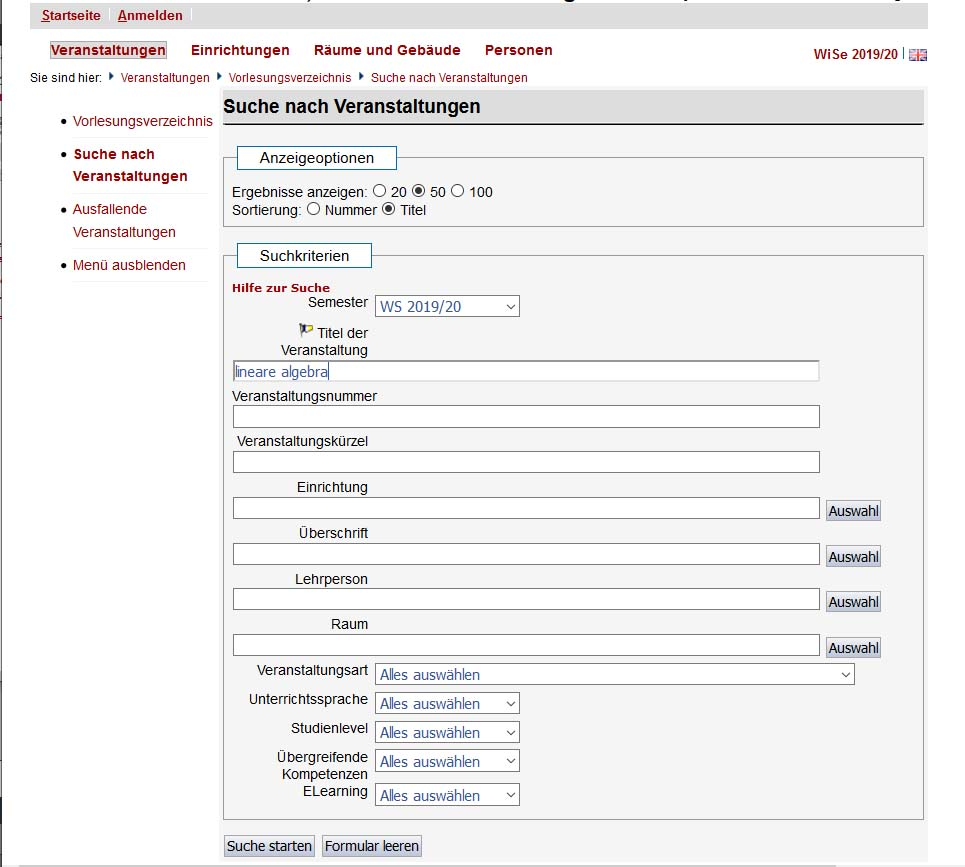
\includegraphics[scale=0.25]{images/lsf09.jpg}
    \end{figure}
\end{frame}

\begin{frame}{Veranstaltungssuche über die Suchfunktion}
    \begin{figure}
       \centering
       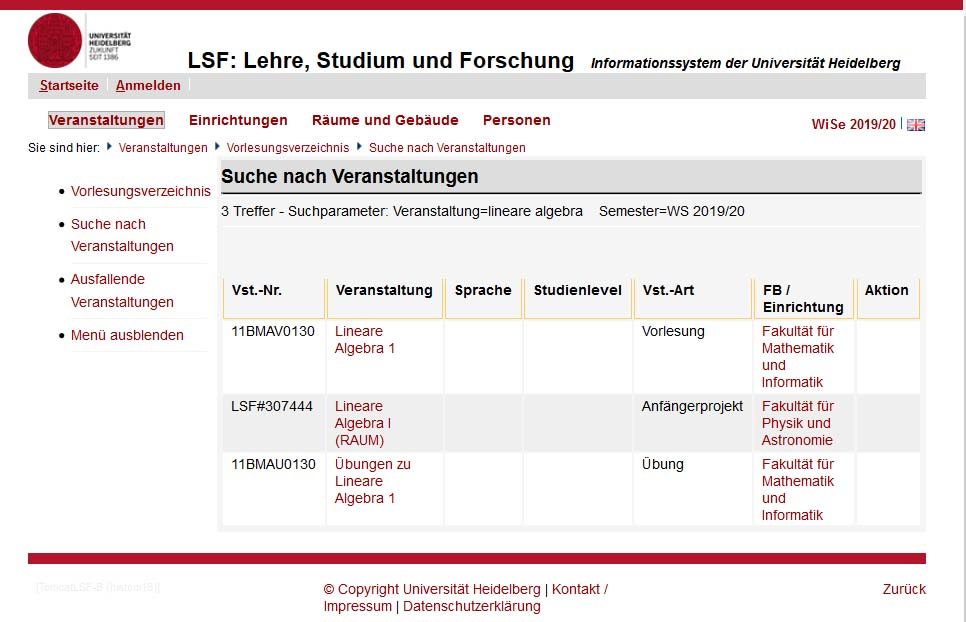
\includegraphics[scale=0.3]{images/lsf10.jpg}
    \end{figure}
\end{frame}

\begin{frame}{Studienbescheinigung, Bafög und Rückmeldung}
    Für diese Funktionen müsst ihr euch anmelden.
    \begin{figure}
        \centering
        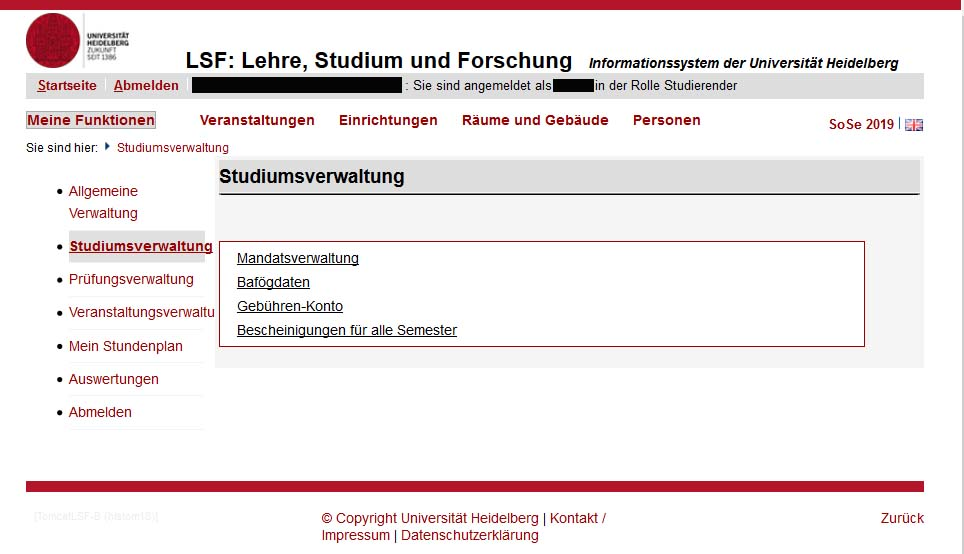
\includegraphics[scale=0.3]{images/lsf12.jpg}
    \end{figure}
\end{frame}

\begin{frame}{Rückmeldung}
    \begin{itemize}
        \item{Erforderlich, wenn ihr weiter studieren wollt}
        \item{Rückmeldung = Semesterbeiträge bezahlen}
        \item{Aufforderung dazu: über die Uni-Mail-Adresse jeweils Mitte Januar und Mitte Juni}
    \end{itemize}
\end{frame}

\begin{frame}{Noten}
    \begin{figure}
        \centering
        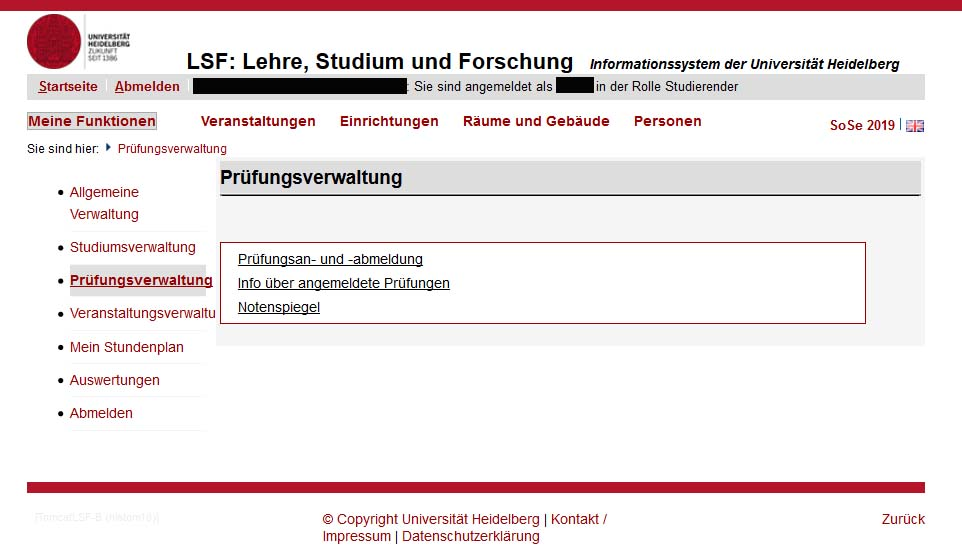
\includegraphics[scale=0.3]{images/lsf13.jpg}
    \end{figure}
    Eure Noten werden - mit etwas Verzögerung - vom jeweiligen fachinternen System hierher übertragen. Auch hierfür müsst ihr euch anmelden.
\end{frame}

\begin{frame}{Studenplan}
    \begin{figure}
        \centering
        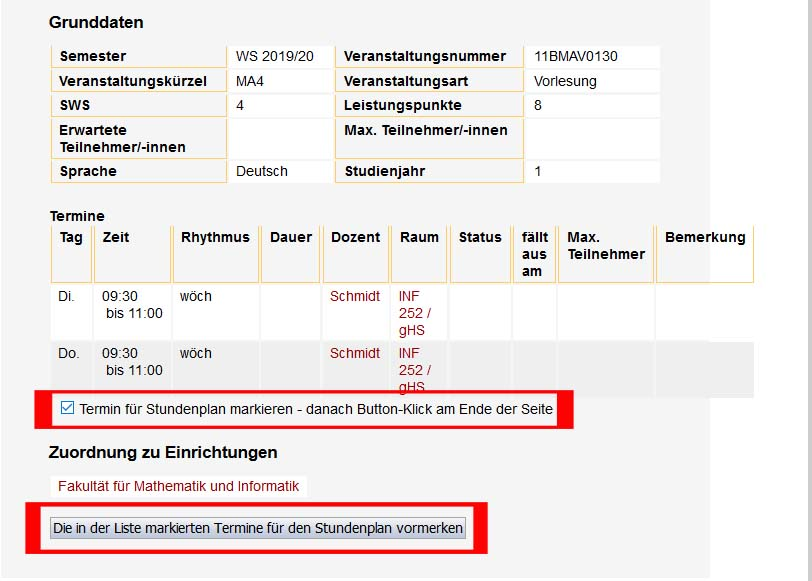
\includegraphics[scale=0.3]{images/lsf14.jpg}
    \end{figure}
    Achtung! Auf diese Weise meldet ihr euch NICHT für Kurse an.
\end{frame}

\begin{frame}{Studenplan}
    \begin{figure}
        \centering
        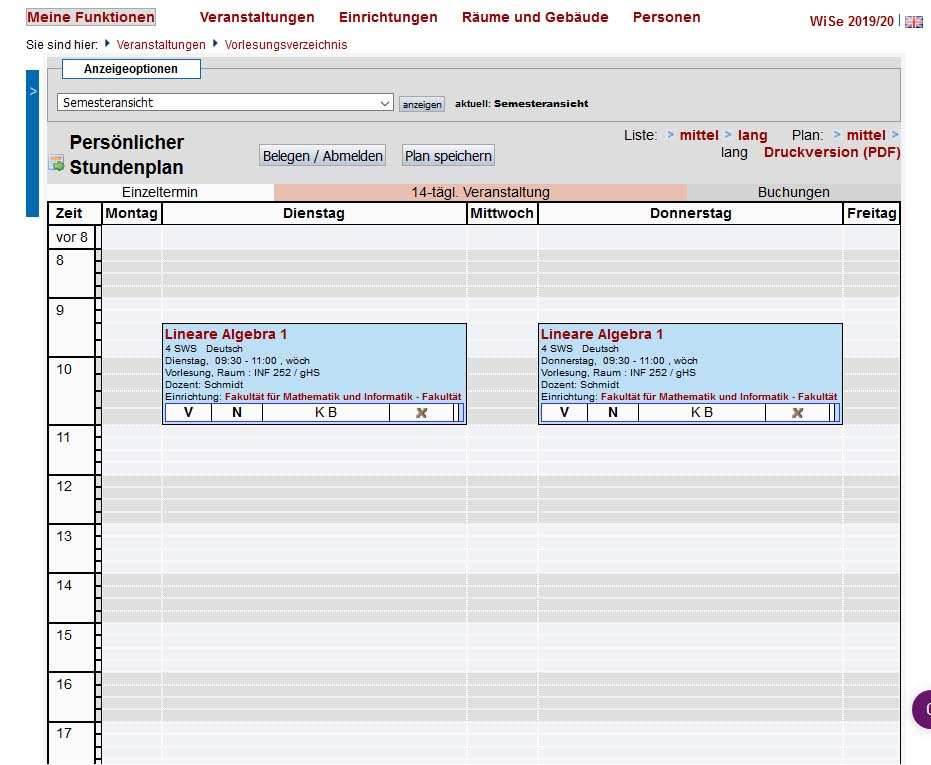
\includegraphics[scale=0.25]{images/lsf15.jpg}
    \end{figure}
\end{frame}

%%%%%%%%%%%%%%%%%%%%%%%%%%%%%%%%%%%%%%%%%%%%%%%%%%%%%%%%%%%%
% MÜSLI
%%%%%%%%%%%%%%%%%%%%%%%%%%%%%%%%%%%%%%%%%%%%%%%%%%%%%%%%%%%%

\subsection{MÜSLI}
\begin{frame}{MÜSLI - Mathematisches Übungsgruppen- und Scheinlisten-Interface}

    \url{https://muesli.mathi.uni-heidelberg.de/}

    \begin{center}
        \qrcode{https://muesli.mathi.uni-heidelberg.de/}
    \end{center}

    \begin{itemize}
        \item{Eintragung in Übungsgruppen (auf diese Weise meldet ihr euch in der Mathe i.d.R. für Veranstaltungen an)}
        \item{Einsehen von Zettelpunkten}
        \item{E-Mail-Adressen der Tutor*innen}
        \item{Klausuranmeldung}
        \item{Noten}
    \end{itemize}
\end{frame}

\begin{frame}{MÜSLI - Mathematisches Übungsgruppen- und Scheinlisten-Interface}
    ACHTUNG!\\
    \begin{enumerate}
        \item{Ihr müsst euch mit eurer Uni-Mail-Adresse registrieren.}
        \item{In anderen Fächern gibt es andere Anmeldemodalitäten. Wenn ihr Kurse in einem anderen Fach belegen wollt/müsst, informiert euch frühzeitig(!) darüber, wie ihr euch in diesem Fach zu Veranstaltungen anmelden könnt.}
    \end{enumerate}
\end{frame}

%%%%%%%%%%%%%%%%%%%%%%%%%%%%%%%%%%%%%%%%%%%%%%%%%%%%%%%%%%%%
% Moodle
%%%%%%%%%%%%%%%%%%%%%%%%%%%%%%%%%%%%%%%%%%%%%%%%%%%%%%%%%%%%

\subsection{Moodle}
\begin{frame}{Moodle - E-Learningplattform}

    \url{https://elearning2.uni-heidelberg.de/}

    \begin{center}
        \qrcode{https://elearning2.uni-heidelberg.de/}
    \end{center}

    \begin{itemize}
        \item{Kurse, in die ihr euch mit einem Einschreibeschlüssel eintragen könnt; Dozent*innen geben den Einschreibeschlüssel i.d.R. in der ersten Sitzung bekannt}
        \item{Materialien zu Veranstaltungen wie Übungsblätter oder Präsentationen}
        \item{Abgaben}
    \end{itemize}

\end{frame}

%%%%%%%%%%%%%%%%%%%%%%%%%%%%%%%%%%%%%%%%%%%%%%%%%%%%%%%%%%%%
% MaMpf
%%%%%%%%%%%%%%%%%%%%%%%%%%%%%%%%%%%%%%%%%%%%%%%%%%%%%%%%%%%%

\subsection{MaMpf}
\begin{frame}{MaMpf - Mathematische Medienplattform}

    \url{https://mampf.mathi.uni-heidelberg.de/}

    \begin{center}
        \qrcode{https://mampf.mathi.uni-heidelberg.de/}
    \end{center}

\end{frame}

%%%%%%%%%%%%%%%%%%%%%%%%%%%%%%%%%%%%%%%%%%%%%%%%%%%%%%%%%%%%
% Software/Anleitungen
%%%%%%%%%%%%%%%%%%%%%%%%%%%%%%%%%%%%%%%%%%%%%%%%%%%%%%%%%%%%

\section{Software \& Anleitungen}
\begin{frame}{Software/Anleitungen}
\end{frame}

%%%%%%%%%%%%%%%%%%%%%%%%%%%%%%%%%%%%%%%%%%%%%%%%%%%%%%%%%%%%
% UB
%%%%%%%%%%%%%%%%%%%%%%%%%%%%%%%%%%%%%%%%%%%%%%%%%%%%%%%%%%%%

\section{Unibibliothek}
\begin{frame}{Unibibliothek}
\end{frame}

%%%%%%%%%%%%%%%%%%%%%%%%%%%%%%%%%%%%%%%%%%%%%%%%%%%%%%%%%%%%
% Fachschaftsservices
%%%%%%%%%%%%%%%%%%%%%%%%%%%%%%%%%%%%%%%%%%%%%%%%%%%%%%%%%%%%

\section{Fachschaftsservices}
\begin{frame}{Fachschaftsservices}
\end{frame}

\end{document}
